% Figure 2.2 (Session 2): exact diagonalization of the Heisenberg chain of L = 4 in three steps.
% The image is rendered by figures/blender/s2_2_ed_recipe.py; the coordinates of the labels
% come from figures/blender/out/ed_recipe_anchors.tex. Compile with:
%   pdflatex ed_recipe.tex ; result moves to ../quantum_magnetism/ed_recipe.pdf
\documentclass[11pt,tikz,border=0pt]{standalone}
\usepackage{amsmath,amssymb,graphicx,braket}
\usepackage{xcolor}
\definecolor{coursedark}{HTML}{1B2A4A}
\definecolor{costamber}{HTML}{B8620A}
\definecolor{diaggreen}{HTML}{1E8C46}
\definecolor{flipcyan}{HTML}{3E4A63}
\newlength{\figw}\setlength{\figw}{16.19cm}   % the text width of the notes (letter, 2.7 cm margins), so labels print at size

\begin{document}
\begin{tikzpicture}[lbl/.style={font=\small, text=coursedark}]
  \node[anchor=south west, inner sep=0pt] at (0,0)
    {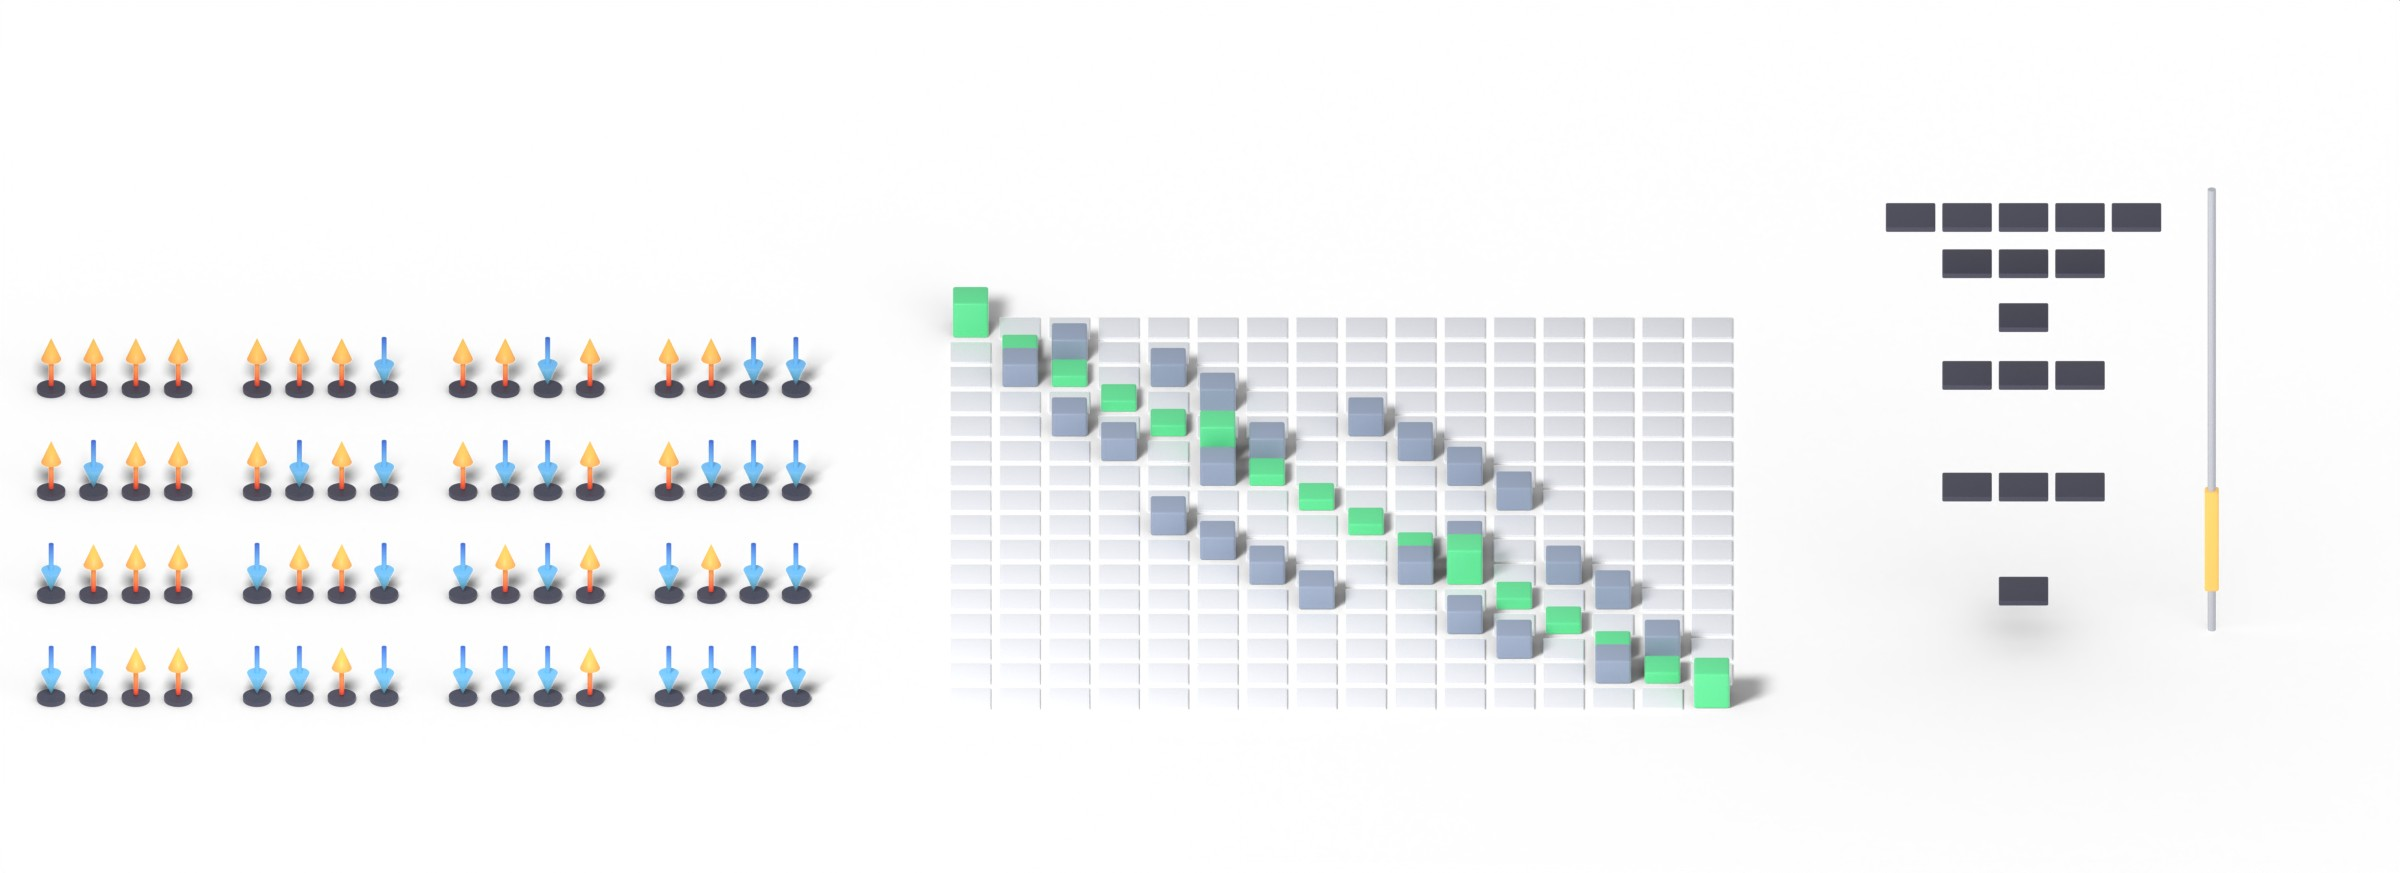
\includegraphics[width=\figw]{../blender/out/ed_recipe.jpg}};
  %% written by figlib.py; x and y in units of the image width
\coordinate (a) at (0.0000\figw,0.2987\figw);
\coordinate (labA) at (0.1765\figw,0.0537\figw);
\coordinate (b) at (0.3676\figw,0.2987\figw);
\coordinate (labB) at (0.5588\figw,0.0537\figw);
\coordinate (diag) at (0.7255\figw,0.0848\figw);
\coordinate (Eaxis) at (0.9216\figw,0.2848\figw);
\coordinate (E0) at (0.8275\figw,0.1177\figw);
\coordinate (E1) at (0.8039\figw,0.1610\figw);
\coordinate (gap) at (0.9216\figw,0.1391\figw);
\coordinate (c) at (0.7304\figw,0.2987\figw);
\coordinate (labC) at (0.8431\figw,0.0537\figw);

  \node[lbl, font=\normalsize, anchor=west] at (a) {(a)};
  \node[lbl, font=\normalsize, anchor=west] at (b) {(b)};
  \node[lbl, font=\normalsize, anchor=west] at (c) {(c)};
  \node[lbl, anchor=north, align=center] at (labA) {the $2^4=16$ product states\\ $\ket{\sigma_1\sigma_2\sigma_3\sigma_4}$};
  \node[lbl, anchor=north, align=center] at (labB)
    {{\color{diaggreen}$S^z_iS^z_{i+1}$} on the diagonal\\
     {\color{flipcyan}$\tfrac12(S^+_iS^-_{i+1}+\mathrm{h.c.})$} off it};
  \node[lbl, anchor=north, align=center] at (labC) {the $16$ eigenvalues\\ \phantom{$\ket{\sigma}$}};
  \node[lbl, anchor=east] at (E0) {$E_0$};
  \node[lbl, anchor=east] at (E1) {$E_1$};
  \node[lbl, text=costamber, anchor=west, xshift=3pt] at (gap) {$\Delta$};
  \node[lbl, anchor=south] at (Eaxis) {$E$};
\end{tikzpicture}
\end{document}
